\section{Introduction}
\label{sec:introduction}

A classifier can predict observed labels accurately while the data weakly distinguish a specified task effect from admissible nuisance variation. This ambiguity matters for classification when statistically similar alternatives prescribe different labels. Autonomous bird monitoring provides a practical motivation: species classifiers operate under variable illumination and occlusion \citep{mansouri2025autonomous}. We ask when it creates a learning obstacle, and how to audit the remaining task information on predefined and learned populations. Group-robust learning and error-based reweighting emphasize subpopulation performance \citep{sagawa2019distributionally,liu2021just}; our objective is to establish which information claims the data support and assess their relevance through controlled nuisance interventions (Figure~\ref{fig:concept}).

Efficient-score projection removes task variation that nuisance scores can reproduce \citep{bickel1993efficient,tsiatis2006semiparametric}. The Fisher-glass framework of \mbox{\citet{mansouri_arai_2026_fisher_glasses}} connects this geometry to inverse-information tails and a population certificate. We develop its classification consequence: decision separation turns limited distinguishability into excess-risk bounds. A worked regression family shows that constant raw information at a reference parameter can conceal an effective sample size set by the mass near the decision boundary. Statistical corrections then determine which population information statements survive estimation error, regularization, and adaptive selection.

\begin{samepage}
On Waterbirds, a frozen feature-based rule selects a group with 92.0\% source accuracy and a 52.6-point controlled drop between same-type and opposite-type background replacements. The information, accuracy, and negative log-likelihood (NLL) selectors identify the same eligible group, whose controlled accuracy drop quantifies background sensitivity. Within that group, nuisance-derived coordinates improve species-held-out prediction of intervention failures beyond a specified confidence baseline. A separate search discovers an accurate population with low predictive information; its sensitivity to interventions remains untested.\par
\end{samepage}

\begin{figure}[t]
\centering
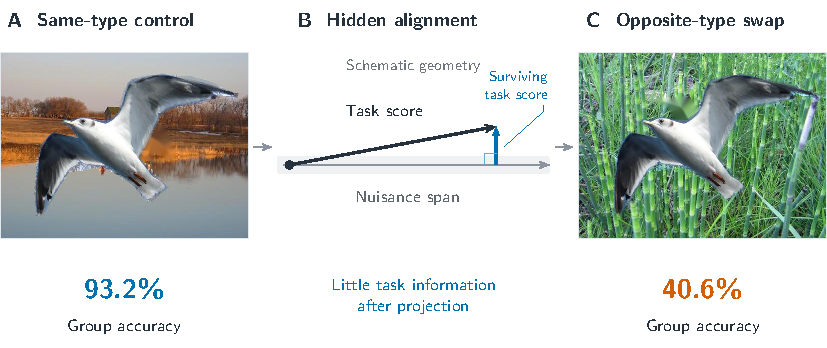
\includegraphics[width=\linewidth]{figures/fig01_concept.pdf}
\caption[High accuracy with weak task information]{\textbf{High accuracy with weak task information.}
(A) Same-type background control: 93.2\% group accuracy. (B) Schematic task--nuisance alignment leaves little information after projection. (C) Opposite-type background swap: 40.6\%, a 52.6-point decrease. Images show one matched example using the same extracted bird foreground and label; accuracies are five-seed means for the selected waterbird/water group.
}
\label{fig:concept}
\end{figure}

Our contributions are:
\begin{itemize}
\item \textbf{A classification consequence.} We derive local excess-risk bounds with explicit decision separation and radius, and exhibit a classification family with matching minimax rates and an interpretable loss of effective sample size.
\item \textbf{Population information audits.} We account for estimation error, ridge bias, membership normalization, and support correction, and evaluate frozen learned slices independently. The audit distinguishes supported information floors from uncertain or adaptively selected estimates.
\item \textbf{Behavioral evaluation.} Controlled interventions and confidence-baseline comparisons test the relevance of nuisance-derived measurements. Training and acquisition evaluate whether information gains correspond to predictive gains, which need not occur together.
\end{itemize}
